\documentclass[14pt]{extbook}
\usepackage{multicol, enumerate, enumitem, hyperref, color, soul, setspace, parskip, fancyhdr} %General Packages
\usepackage{amssymb, amsthm, amsmath, latexsym, units, mathtools} %Math Packages
\everymath{\displaystyle} %All math in Display Style
% Packages with additional options
\usepackage[headsep=0.5cm,headheight=12pt, left=1 in,right= 1 in,top= 1 in,bottom= 1 in]{geometry}
\usepackage[usenames,dvipsnames]{xcolor}
\usepackage{dashrule}  % Package to use the command below to create lines between items
\newcommand{\litem}[1]{\item#1\hspace*{-1cm}\rule{\textwidth}{0.4pt}}
\pagestyle{fancy}
\lhead{Progress Quiz 8}
\chead{}
\rhead{Version B}
\lfoot{5493-4176}
\cfoot{}
\rfoot{Summer C 2021}
\begin{document}

\begin{enumerate}
\litem{
Determine the horizontal and/or oblique asymptotes in the rational function below.\[ f(x) = \frac{8x^{3} +10 x^{2} -9 x -9}{4x^{2} +23 x + 15} \]\begin{enumerate}[label=\Alph*.]
\item \( \text{Horizontal Asymptote at } y = -5.0 \)
\item \( \text{Horizontal Asymptote of } y = -5.0 \text{ and Oblique Asymptote of } y = 2x -9 \)
\item \( \text{Oblique Asymptote of } y = 2x -9. \)
\item \( \text{Horizontal Asymptote of } y = 2.0 \text{ and Oblique Asymptote of } y = 2x -9 \)
\item \( \text{Horizontal Asymptote of } y = 2.0  \)

\end{enumerate} }
\litem{
Determine the vertical asymptotes and holes in the rational function below.\[ f(x) = \frac{8x^{3} +38 x^{2} +15 x -36}{16x^{2} +8 x -15} \]\begin{enumerate}[label=\Alph*.]
\item \( \text{Holes at } x = -1.25 \text{ and } x = 0.75 \text{ with no vertical asymptotes.} \)
\item \( \text{Vertical Asymptote of } x = -1.25 \text{ and hole at } x = 0.75 \)
\item \( \text{Vertical Asymptotes of } x = -1.25 \text{ and } x = -1.5 \text{ with a hole at } x = 0.75 \)
\item \( \text{Vertical Asymptote of } x = 0.5 \text{ and hole at } x = 0.75 \)
\item \( \text{Vertical Asymptotes of } x = -1.25 \text{ and } x = 0.75 \text{ with no holes.} \)

\end{enumerate} }
\litem{
Determine the horizontal and/or oblique asymptotes in the rational function below.\[ f(x) = \frac{6x^{3} -29 x^{2} +43 x -20}{-4x^{3} +28 x^{2} -38 x + 20} \]\begin{enumerate}[label=\Alph*.]
\item \( \text{Vertical Asymptote of } y = 2.000  \)
\item \( \text{Horizontal Asymptote of } y = 0  \)
\item \( \text{Horizontal Asymptote of } y = -1.500  \)
\item \( \text{None of the above} \)
\item \( \text{Vertical Asymptote of } y = 1  \)

\end{enumerate} }
\litem{
Which of the following functions \textit{could} be the graph below?
\begin{center}
    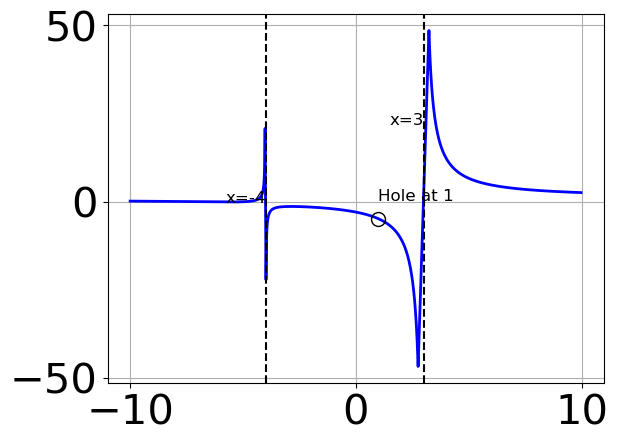
\includegraphics[width=0.5\textwidth]{../Figures/identifyGraphOfRationalFunctionB.png}
\end{center}
\begin{enumerate}[label=\Alph*.]
\item \( f(x)=\frac{x^{3} +11.0 x^{2} +23.0 x -35.0}{x^{3} -13.0 x + 12.0} \)
\item \( f(x)=\frac{x^{3} -5.0 x^{2} -49.0 x + 245.0}{x^{3} -13.0 x -12.0} \)
\item \( f(x)=\frac{x^{3} -11.0 x^{2} +23.0 x + 35.0}{x^{3} -13.0 x -12.0} \)
\item \( f(x)=\frac{x^{3} +18.0 x^{2} +107.0 x + 210.0}{x^{3} -13.0 x + 12.0} \)
\item \( \text{None of the above are possible equations for the graph.} \)

\end{enumerate} }
\litem{
Determine the vertical asymptotes and holes in the rational function below.\[ f(x) = \frac{12x^{3} -1 x^{2} -38 x + 24}{8x^{2} -18 x + 9} \]\begin{enumerate}[label=\Alph*.]
\item \( \text{Vertical Asymptotes of } x = 1.5 \text{ and } x = 0.75 \text{ with no holes.} \)
\item \( \text{Holes at } x = 1.5 \text{ and } x = 0.75 \text{ with no vertical asymptotes.} \)
\item \( \text{Vertical Asymptotes of } x = 1.5 \text{ and } x = 1.333 \text{ with a hole at } x = 0.75 \)
\item \( \text{Vertical Asymptote of } x = 1.5 \text{ and hole at } x = 0.75 \)
\item \( \text{Vertical Asymptote of } x = 1.5 \text{ and hole at } x = 0.75 \)

\end{enumerate} }
\litem{
Determine the horizontal and/or oblique asymptotes in the rational function below.\[ f(x) = \frac{6x^{3} -31 x^{2} +48 x -20}{3x^{2} -14 x + 8} \]\begin{enumerate}[label=\Alph*.]
\item \( \text{Horizontal Asymptote of } y = 4.0 \text{ and Oblique Asymptote of } y = 2x -1 \)
\item \( \text{Horizontal Asymptote at } y = 4.0 \)
\item \( \text{Oblique Asymptote of } y = 2x -1. \)
\item \( \text{Horizontal Asymptote of } y = 2.0 \text{ and Oblique Asymptote of } y = 2x -1 \)
\item \( \text{Horizontal Asymptote of } y = 2.0  \)

\end{enumerate} }
\litem{
Determine the horizontal and/or oblique asymptotes in the rational function below.\[ f(x) = \frac{6x^{2} +13 x -15}{18x^{3} -9 x^{2} -17 x + 10} \]\begin{enumerate}[label=\Alph*.]
\item \( \text{Horizontal Asymptote of } y = 0.333 \text{ and Oblique Asymptote of } y = 3x -8 \)
\item \( \text{Oblique Asymptote of } y = 3x -8. \)
\item \( \text{Horizontal Asymptote of } y = 0.333  \)
\item \( \text{Horizontal Asymptote of } y = 0 \)
\item \( \text{Horizontal Asymptote at } y = -3.000 \)

\end{enumerate} }
\litem{
Which of the following functions \textit{could} be the graph below?
\begin{center}
    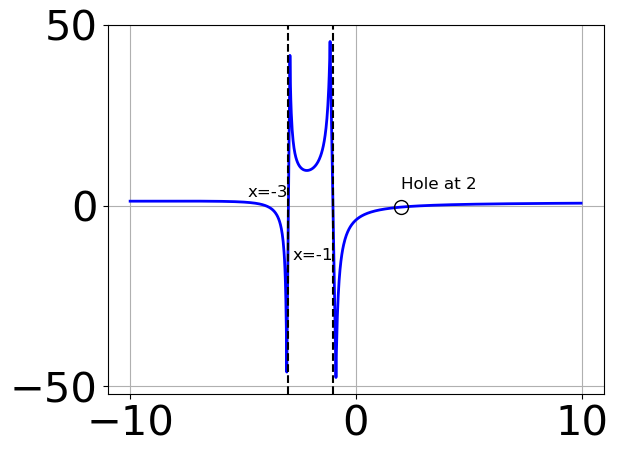
\includegraphics[width=0.5\textwidth]{../Figures/identifyGraphOfRationalFunctionCopyB.png}
\end{center}
\begin{enumerate}[label=\Alph*.]
\item \( f(x)=\frac{x^{3} + x^{2} -14.0 x -24.0}{x^{3} -2.0 x^{2} -5.0 x + 6.0} \)
\item \( f(x)=\frac{x^{3} -4.0 x^{2} -17.0 x + 60.0}{x^{3} +2.0 x^{2} -5.0 x -6.0} \)
\item \( f(x)=\frac{x^{3} -1.0 x^{2} -14.0 x + 24.0}{x^{3} +2.0 x^{2} -5.0 x -6.0} \)
\item \( f(x)=\frac{x^{3} -7.0 x^{2} -6.0 x + 72.0}{x^{3} -2.0 x^{2} -5.0 x + 6.0} \)
\item \( \text{None of the above are possible equations for the graph.} \)

\end{enumerate} }
\litem{
Determine the vertical asymptotes and holes in the rational function below.\[ f(x) = \frac{8x^{3} -42 x^{2} +63 x -27}{6x^{2} -5 x -6} \]\begin{enumerate}[label=\Alph*.]
\item \( \text{Vertical Asymptotes of } x = -0.667 \text{ and } x = 1.5 \text{ with no holes.} \)
\item \( \text{Holes at } x = -0.667 \text{ and } x = 1.5 \text{ with no vertical asymptotes.} \)
\item \( \text{Vertical Asymptotes of } x = -0.667 \text{ and } x = 0.75 \text{ with a hole at } x = 1.5 \)
\item \( \text{Vertical Asymptote of } x = 1.333 \text{ and hole at } x = 1.5 \)
\item \( \text{Vertical Asymptote of } x = -0.667 \text{ and hole at } x = 1.5 \)

\end{enumerate} }
\litem{
Determine the vertical asymptotes and holes in the rational function below.\[ f(x) = \frac{6x^{3} -19 x^{2} -45 x + 100}{9x^{2} -21 x + 10} \]\begin{enumerate}[label=\Alph*.]
\item \( \text{Vertical Asymptote of } x = 0.667 \text{ and hole at } x = 1.667 \)
\item \( \text{Vertical Asymptote of } x = 0.667 \text{ and hole at } x = 1.667 \)
\item \( \text{Holes at } x = 0.667 \text{ and } x = 1.667 \text{ with no vertical asymptotes.} \)
\item \( \text{Vertical Asymptotes of } x = 0.667 \text{ and } x = -2.5 \text{ with a hole at } x = 1.667 \)
\item \( \text{Vertical Asymptotes of } x = 0.667 \text{ and } x = 1.667 \text{ with no holes.} \)

\end{enumerate} }
\end{enumerate}

\end{document}